% !TeX root = ../tfg.tex
% !TeX encoding = utf8
%
%*******************************************************
% Capítulo 12. Predicción conforme
%*******************************************************

\chapter{Predicción conforme}\label{cap:conforme}

% Esqueleto: las notas no incluyen texto de este capítulo. Cifras de results_conforme/ y
% results_conforme/mondrian/. Fundamentos en la \cref{sec:prediccion-conforme}.
% Limitación común: la validación ID se usó durante el entrenamiento para elegir la época
% (EarlyStoppingCallback sobre valid_loss) y procede de la carpeta train original, mientras que el
% test procede de la carpeta val original; la intercambiabilidad no está asegurada. Exactitud del
% Swin-S: 97,02 % en validación y 96,88 % en test.
\pendiente{introducción del capítulo y limitación de intercambiabilidad entre validación y test}

\section{Detección OOD conforme}\label{sec:conforme-ood}

% Puntos que debería cubrir:
% - Umbral calibrado con las puntuaciones de la validación ID (n = 22.691):
%   p(x) = (1 + #\{s_i \le s(x)\}) / (n + 1); OOD si p(x) \le \alpha.
% - Falsas alarmas en el test ID compatibles con \alpha en los 15 casos (5 métodos x 3 valores de
%   \alpha): el IC exacto contiene \alpha en todos.
% - Con \alpha = 0,05: STOOD-X es el que más detecta en TUM+NORM (0,879), PANDA (0,568) y DTD (0,972),
%   a diferencia de lo que indicaba FPR@95 (otro punto de funcionamiento); también el que más marca
%   el control de resolución (0,596). ViM y MDS detectan más LYM (0,826 y 0,813).
% - Con \alpha = 0,01, ViM y MDS detectan ~55 % de TUM+NORM y STOOD-X el 75 %.
\pendiente{análisis de la \cref{tab:conforme-ood}}

% Generado por scripts/generar_tablas.py a partir de results_conforme/deteccion_ood_conforme.csv. No editar a mano.
\begin{table}[htbp]
\centering
\scriptsize
\setlength{\tabcolsep}{3pt}
\caption{Detección OOD conforme con el umbral calibrado en la validación ID (22.691 imágenes). Falsas alarmas: proporción del test ID marcada como OOD, con IC exacto del 95\,\% (debe ser compatible con $\alpha$ si validación y test son intercambiables). Resto de columnas: proporción detectada como OOD en cada conjunto (más alto es mejor).}
\label{tab:conforme-ood}
\begin{tabular}{llcccccc}
\toprule
Método & $\alpha$ & Falsas alarmas test ID [IC 95\,\%] & TUM+NORM & LYM & PANDA & Control 128\,px & DTD \\
\midrule
MSP & 0{,}01 & 0{,}009 [0{,}008; 0{,}011] & 0{,}261 & 0{,}203 & 0{,}072 & 0{,}033 & 0{,}158 \\
 & 0{,}05 & 0{,}050 [0{,}046; 0{,}054] & 0{,}631 & 0{,}576 & 0{,}392 & 0{,}134 & 0{,}509 \\
 & 0{,}10 & 0{,}098 [0{,}093; 0{,}103] & 0{,}794 & 0{,}749 & 0{,}695 & 0{,}277 & 0{,}771 \\
\midrule
ViM & 0{,}01 & 0{,}010 [0{,}008; 0{,}012] & 0{,}552 & 0{,}569 & 0{,}110 & 0{,}077 & 0{,}437 \\
 & 0{,}05 & 0{,}049 [0{,}045; 0{,}053] & 0{,}796 & 0{,}826 & 0{,}448 & 0{,}209 & 0{,}721 \\
 & 0{,}10 & 0{,}099 [0{,}094; 0{,}105] & 0{,}902 & 0{,}886 & 0{,}646 & 0{,}324 & 0{,}857 \\
\midrule
MDS & 0{,}01 & 0{,}010 [0{,}009; 0{,}012] & 0{,}554 & 0{,}554 & 0{,}118 & 0{,}077 & 0{,}431 \\
 & 0{,}05 & 0{,}049 [0{,}046; 0{,}053] & 0{,}786 & 0{,}812 & 0{,}448 & 0{,}201 & 0{,}707 \\
 & 0{,}10 & 0{,}099 [0{,}094; 0{,}104] & 0{,}892 & 0{,}878 & 0{,}637 & 0{,}312 & 0{,}843 \\
\midrule
RMDS & 0{,}01 & 0{,}010 [0{,}008; 0{,}011] & 0{,}359 & 0{,}348 & 0{,}184 & 0{,}043 & 0{,}173 \\
 & 0{,}05 & 0{,}052 [0{,}048; 0{,}056] & 0{,}694 & 0{,}606 & 0{,}430 & 0{,}150 & 0{,}542 \\
 & 0{,}10 & 0{,}098 [0{,}093; 0{,}103] & 0{,}897 & 0{,}725 & 0{,}700 & 0{,}297 & 0{,}818 \\
\midrule
STOOD-X 100 \% ($-z$) & 0{,}01 & 0{,}011 [0{,}009; 0{,}013] & 0{,}748 & 0{,}385 & 0{,}272 & 0{,}263 & 0{,}841 \\
 & 0{,}05 & 0{,}049 [0{,}046; 0{,}053] & 0{,}879 & 0{,}671 & 0{,}568 & 0{,}596 & 0{,}972 \\
 & 0{,}10 & 0{,}103 [0{,}097; 0{,}108] & 0{,}889 & 0{,}753 & 0{,}705 & 0{,}724 & 0{,}986 \\
\bottomrule
\end{tabular}
\end{table}


\pendiente{conclusión parcial}

\section{Conjuntos de predicción APS y RAPS}\label{sec:conforme-aps}

% Puntos que debería cubrir:
% - Calibración con el 80 % de la validación ID (18.153); el 20 % restante (4.538) para ajustar RAPS
%   (k_reg = 1, \lambda = 0,5: en la práctica, conjuntos de tamaño 0 o 1).
% - Verificación por simulación de la implementación (1.000 particiones, n = 4.000).
% - Test ID: APS \alpha = 0,05: cobertura 0,945 [0,941; 0,949], tamaño 1,04, vacíos 3,9 %; el déficit
%   de 0,005 es de ~1,9 desviaciones típicas.
% - Conjuntos vacíos: como la exactitud supera 1 - \alpha, el método puede «abstenerse».
% - Control de resolución: la garantía se rompe (APS 0,922 y RAPS 0,894 con \alpha = 0,05).
\pendiente{análisis de la \cref{tab:conforme-aps} y de la \cref{fig:conforme-cobertura}}

% Generado por scripts/generar_tablas.py a partir de results_conforme/aps_raps_resumen.csv. No editar a mano.
\begin{table}[tbp]
\centering
\footnotesize
\setlength{\tabcolsep}{3pt}
\caption{Conjuntos de predicción APS y RAPS sobre las probabilidades del Swin-S, calibrados con el 80\,\% de la validación ID. Cobertura: proporción de imágenes cuya clase verdadera está en el conjunto (objetivo $1-\alpha$), con IC exacto del 95\,\%; tamaño medio del conjunto (más pequeño es mejor a igual cobertura) y proporción de conjuntos vacíos.}
\label{tab:conforme-aps}
\begin{tabular}{llccccc}
\toprule
& & \multicolumn{3}{c}{Test ID} & \multicolumn{2}{c}{Control 128\,px} \\
\cmidrule(lr){3-5}\cmidrule(lr){6-7}
Método & $\alpha$ & Cobertura [IC 95\,\%] & Tamaño & Vacíos & Cobertura & Tamaño \\
\midrule
APS & 0{,}05 & 0{,}945 [0{,}941; 0{,}949] & 1{,}04 & 3{,}9\,\% & 0{,}922 & 1{,}25 \\
RAPS & 0{,}05 & 0{,}948 [0{,}944; 0{,}952] & 0{,}98 & 2{,}1\,\% & 0{,}894 & 0{,}99 \\
APS & 0{,}10 & 0{,}897 [0{,}892; 0{,}902] & 0{,}95 & 8{,}4\,\% & 0{,}871 & 1{,}07 \\
RAPS & 0{,}10 & 0{,}898 [0{,}892; 0{,}903] & 0{,}93 & 7{,}2\,\% & 0{,}852 & 0{,}94 \\
\bottomrule
\end{tabular}
\end{table}


\begin{figure}[tbp]
  \centering
  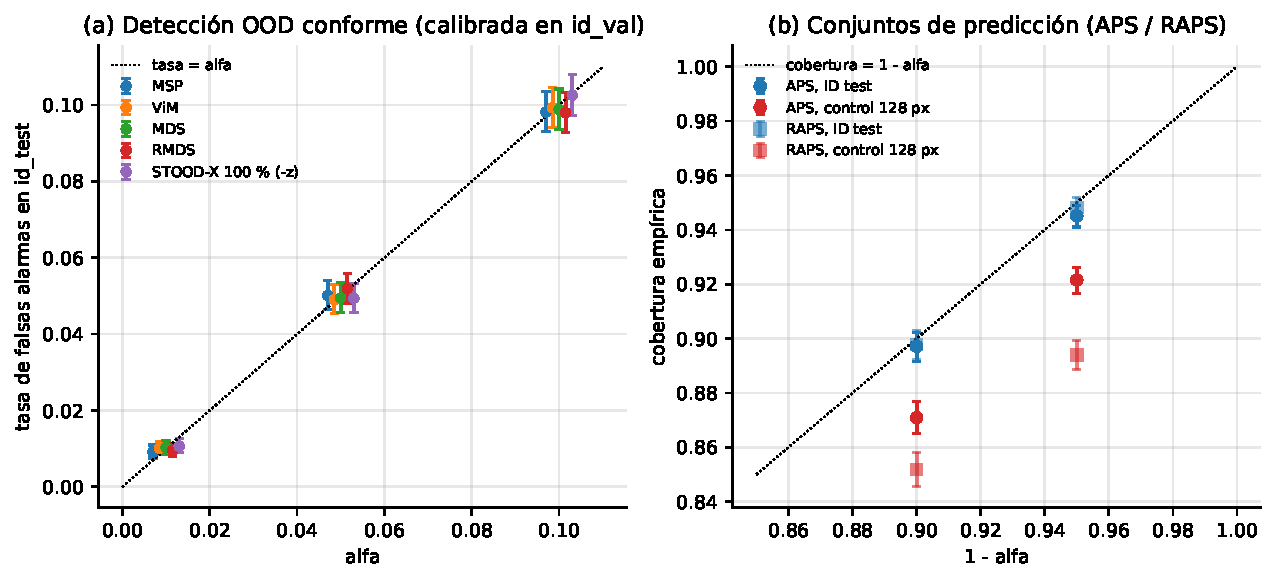
\includegraphics[width=0.8\textwidth]{img/cap12/fig_cobertura.pdf}
  \caption{Cobertura de los conjuntos de predicción APS y RAPS en el test ID y en el control de resolución frente al objetivo $1-\alpha$.}
  \label{fig:conforme-cobertura}
\end{figure}

% Puntos que debería cubrir:
% - La garantía es marginal, no por clase: con \alpha = 0,05, glomeruloide 0,68 (APS) y 0,52 (RAPS);
%   pobremente formadas 0,79 y 0,73; Gleason_3 0,87 y 0,79. APS compensa con conjuntos mayores en
%   esas clases (~1,4 frente a ~1,0).
% - Con APS, el tamaño medio crece fuera de distribución (\alpha = 0,05: 3,14 en TUM+NORM, 2,72 en
%   LYM, 2,51 en DTD, 1,69 en PANDA, frente a 1,04 en el test ID): el tamaño es una señal de OOD.
%   Con RAPS esa señal desaparece.
\pendiente{análisis de la \cref{tab:conforme-tamano-ood} y de la \cref{fig:conforme-tamanos-clase}}

% Generado por scripts/generar_tablas.py a partir de results_conforme/aps_raps_resumen.csv. No editar a mano.
\begin{table}[htbp]
\centering
\scriptsize
\setlength{\tabcolsep}{3pt}
\caption{Tamaño medio de los conjuntos de predicción APS y RAPS en el test ID y en los conjuntos OOD. Un tamaño mayor fuera de distribución indica que el conjunto refleja la incertidumbre ante entradas OOD.}
\label{tab:conforme-tamano-ood}
\begin{tabular}{llcccccccccc}
\toprule
Método & $\alpha$ & Test ID & TUM+NORM & TUM & NORM & STR & LYM & MUS & PANDA & Control 128\,px & DTD \\
\midrule
APS & 0{,}05 & 1{,}04 & 3{,}14 & 3{,}12 & 3{,}16 & 2{,}08 & 2{,}72 & 1{,}74 & 1{,}69 & 1{,}25 & 2{,}51 \\
RAPS & 0{,}05 & 0{,}98 & 1{,}04 & 1{,}04 & 1{,}05 & 1{,}00 & 1{,}02 & 0{,}99 & 0{,}99 & 0{,}99 & 1{,}01 \\
APS & 0{,}10 & 0{,}95 & 2{,}37 & 2{,}34 & 2{,}41 & 1{,}53 & 2{,}00 & 1{,}35 & 1{,}28 & 1{,}07 & 1{,}82 \\
RAPS & 0{,}10 & 0{,}93 & 1{,}00 & 1{,}00 & 1{,}01 & 0{,}96 & 0{,}98 & 0{,}96 & 0{,}96 & 0{,}94 & 0{,}98 \\
\bottomrule
\end{tabular}
\end{table}


\begin{figure}[tbp]
  \centering
  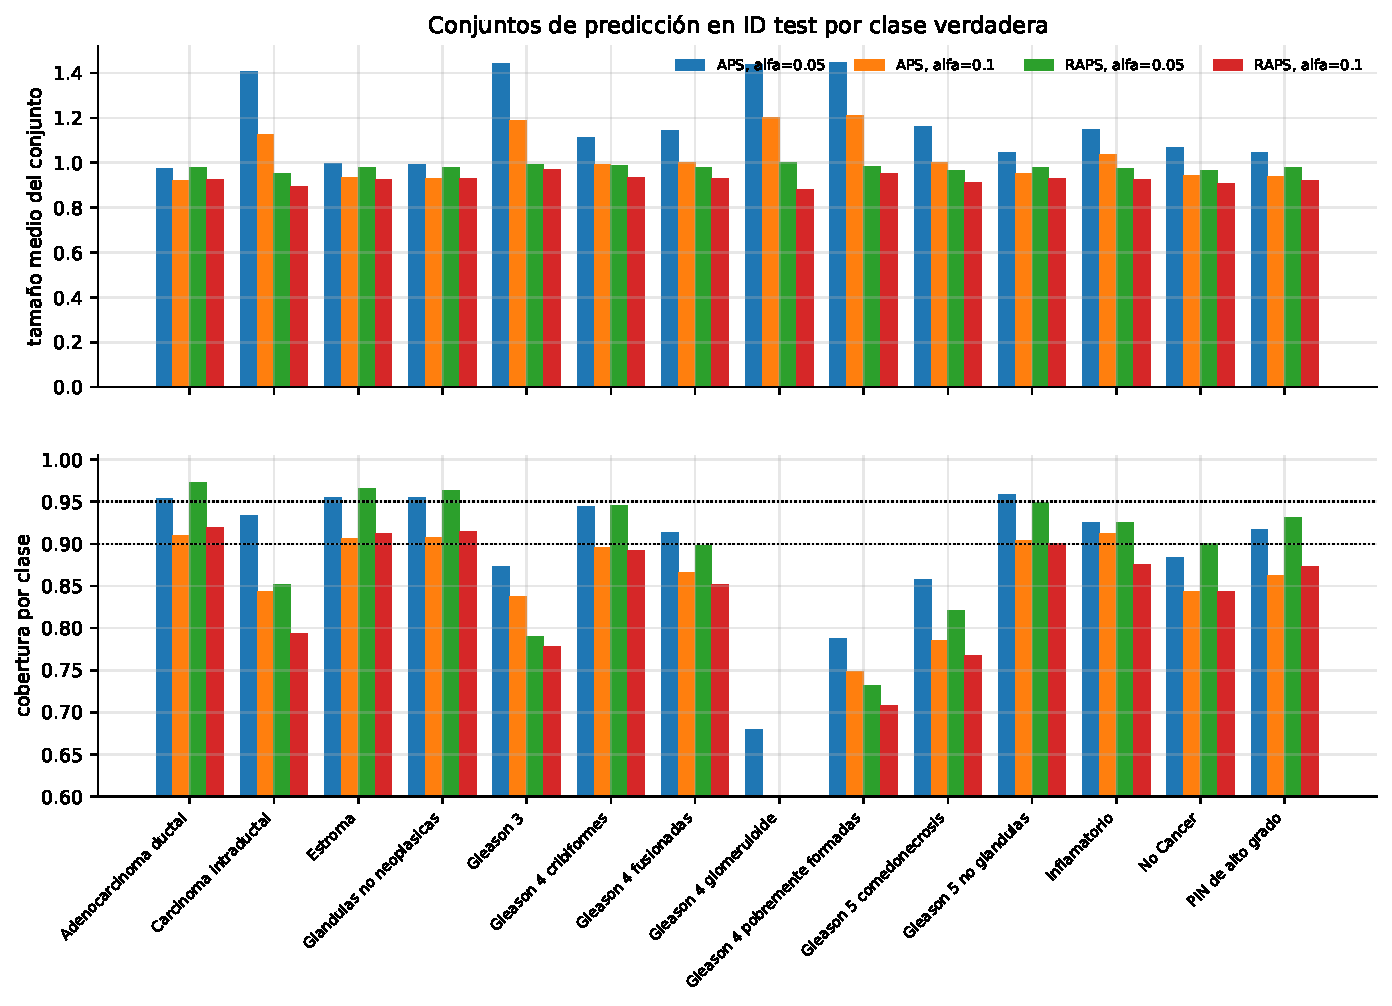
\includegraphics[width=0.8\textwidth]{img/cap12/fig_tamanos_por_clase.pdf}
  \caption{Cobertura y tamaño medio de los conjuntos APS y RAPS por clase en el test ID.}
  \label{fig:conforme-tamanos-clase}
\end{figure}

\pendiente{conclusión parcial}

\section{Predicción conforme Mondrian}\label{sec:conforme-mondrian}

% Puntos que debería cubrir:
% - Puntuaciones LAC (1 - softmax) y APS; misma calibración que la versión marginal.
% - La cobertura global es la misma (LAC \alpha = 0,05: 0,948 en ambas), pero el tamaño medio se
%   duplica con \alpha = 0,05 (LAC 0,96 -> 1,98; APS 1,04 -> 2,15).
% - Control de resolución: ninguna versión mantiene la garantía; con LAC, Mondrian empeora
%   (0,859 -> 0,777).
\pendiente{análisis de la \cref{tab:mondrian-global}}

% Generado por scripts/generar_tablas.py a partir de results_conforme/mondrian/global.csv. No editar a mano.
\begin{table}[tbp]
\centering
\scriptsize
\setlength{\tabcolsep}{3pt}
\caption{Predicción conforme marginal frente a Mondrian (condicionada por clase) con las puntuaciones LAC y APS. Cobertura (objetivo $1-\alpha$) con IC exacto del 95\,\%, tamaño medio del conjunto, número de clases con cobertura puntual por debajo de $1-\alpha$ en el test ID y cobertura en el control de resolución (\emph{covariate shift} con las mismas etiquetas).}
\label{tab:mondrian-global}
\begin{tabular}{lllcccc}
\toprule
Puntuación & $\alpha$ & Versión & Cobertura test ID [IC 95\,\%] & Tamaño medio & Clases $<1-\alpha$ & Cobertura control 128\,px \\
\midrule
APS & 0{,}05 & Marginal & 0{,}945 [0{,}941; 0{,}949] & 1{,}04 & 10 / 14 & 0{,}922 \\
APS & 0{,}05 & Mondrian & 0{,}946 [0{,}942; 0{,}950] & 2{,}15 & 11 / 14 & 0{,}923 \\
\midrule
APS & 0{,}10 & Marginal & 0{,}897 [0{,}892; 0{,}902] & 0{,}95 & 9 / 14 & 0{,}871 \\
APS & 0{,}10 & Mondrian & 0{,}899 [0{,}894; 0{,}904] & 0{,}98 & 10 / 14 & 0{,}874 \\
\midrule
LAC & 0{,}05 & Marginal & 0{,}948 [0{,}944; 0{,}952] & 0{,}96 & 10 / 14 & 0{,}859 \\
LAC & 0{,}05 & Mondrian & 0{,}948 [0{,}944; 0{,}952] & 1{,}98 & 8 / 14 & 0{,}777 \\
\midrule
LAC & 0{,}10 & Marginal & 0{,}901 [0{,}896; 0{,}906] & 0{,}91 & 10 / 14 & 0{,}726 \\
LAC & 0{,}10 & Mondrian & 0{,}901 [0{,}896; 0{,}906] & 0{,}94 & 7 / 14 & 0{,}649 \\
\bottomrule
\end{tabular}
\end{table}


% Puntos que debería cubrir:
% - La versión marginal sobrecubre las clases grandes (0,97-0,99) e infracubre mucho las pequeñas
%   (0,40 en glomeruloide, 0,61 en pobremente formadas); Mondrian iguala la cobertura entre clases.
% - Gleason_4_pobremente_formadas (0,874 [0,803; 0,926]) y Gleason_3 (0,901 [0,858; 0,935]) siguen
%   por debajo de 0,95 con IC que no incluyen 0,95.
\pendiente{análisis de la \cref{tab:mondrian-clase} y de la \cref{fig:mondrian-cobertura-clase}}

% Generado por scripts/generar_tablas.py a partir de results_conforme/mondrian/por_clase.csv. No editar a mano.
\begin{table}[htbp]
\centering
\scriptsize
\setlength{\tabcolsep}{3pt}
\caption{Cobertura por clase en el test ID con la puntuación LAC y $\alpha=0{,}05$: versión marginal frente a Mondrian (objetivo: $0{,}95$ en cada clase). $n_y$: imágenes de calibración de la clase; $k_y=\lceil (n_y+1)(1-\alpha)\rceil$. $^{\max}$: $k_y=n_y$, el umbral es la mayor puntuación de calibración de la clase.}
\label{tab:mondrian-clase}
\begin{tabular}{lrrcccc}
\toprule
& & & \multicolumn{2}{c}{Cobertura} & \multicolumn{2}{c}{Tamaño medio} \\
\cmidrule(lr){4-5}\cmidrule(lr){6-7}
Clase & $n_y$ & $k_y$ & Marginal & Mondrian & Marginal & Mondrian \\
\midrule
\clase{Gleason\_4\_glomeruloide} & \num{33} & \num{33}$^{\max}$ & 0{,}400 & 1{,}000 & 0{,}72 & 1{,}60 \\
\clase{Gleason\_5\_comedonecrosis} & \num{82} & \num{79} & 0{,}804 & 0{,}946 & 0{,}89 & 2{,}11 \\
\clase{Inflamatorio} & \num{113} & \num{109} & 0{,}850 & 1{,}000 & 0{,}86 & 2{,}08 \\
\clase{Carcinoma\_intraductal} & \num{169} & \num{162} & 0{,}793 & 0{,}983 & 0{,}82 & 2{,}03 \\
\clase{Gleason\_4\_pobremente\_formadas} & \num{174} & \num{167} & 0{,}606 & 0{,}874 & 0{,}76 & 2{,}15 \\
\clase{No\_Cancer} & \num{174} & \num{167} & 0{,}901 & 0{,}934 & 0{,}94 & 1{,}98 \\
\clase{Gleason\_3} & \num{359} & \num{342} & 0{,}719 & 0{,}901 & 0{,}83 & 2{,}04 \\
\clase{PIN\_de\_alto\_grado} & \num{391} & \num{373} & 0{,}928 & 0{,}957 & 0{,}96 & 2{,}01 \\
\clase{Gleason\_4\_fusionadas} & \num{1111} & \num{1057} & 0{,}873 & 0{,}943 & 0{,}92 & 2{,}04 \\
\clase{Gleason\_5\_no\_glandulas} & \num{1757} & \num{1671} & 0{,}955 & 0{,}955 & 0{,}96 & 2{,}00 \\
\clase{Gleason\_4\_cribiformes} & \num{2037} & \num{1937} & 0{,}924 & 0{,}944 & 0{,}94 & 2{,}01 \\
\clase{Adenocarcinoma\_ductal} & \num{3020} & \num{2870} & 0{,}992 & 0{,}959 & 0{,}99 & 1{,}97 \\
\clase{Estroma} & \num{3536} & \num{3361} & 0{,}974 & 0{,}945 & 0{,}98 & 1{,}96 \\
\clase{Glandulas\_no\_neoplasicas} & \num{5197} & \num{4939} & 0{,}972 & 0{,}946 & 0{,}98 & 1{,}96 \\
\bottomrule
\end{tabular}
\end{table}


\begin{figure}[tbp]
  \centering
  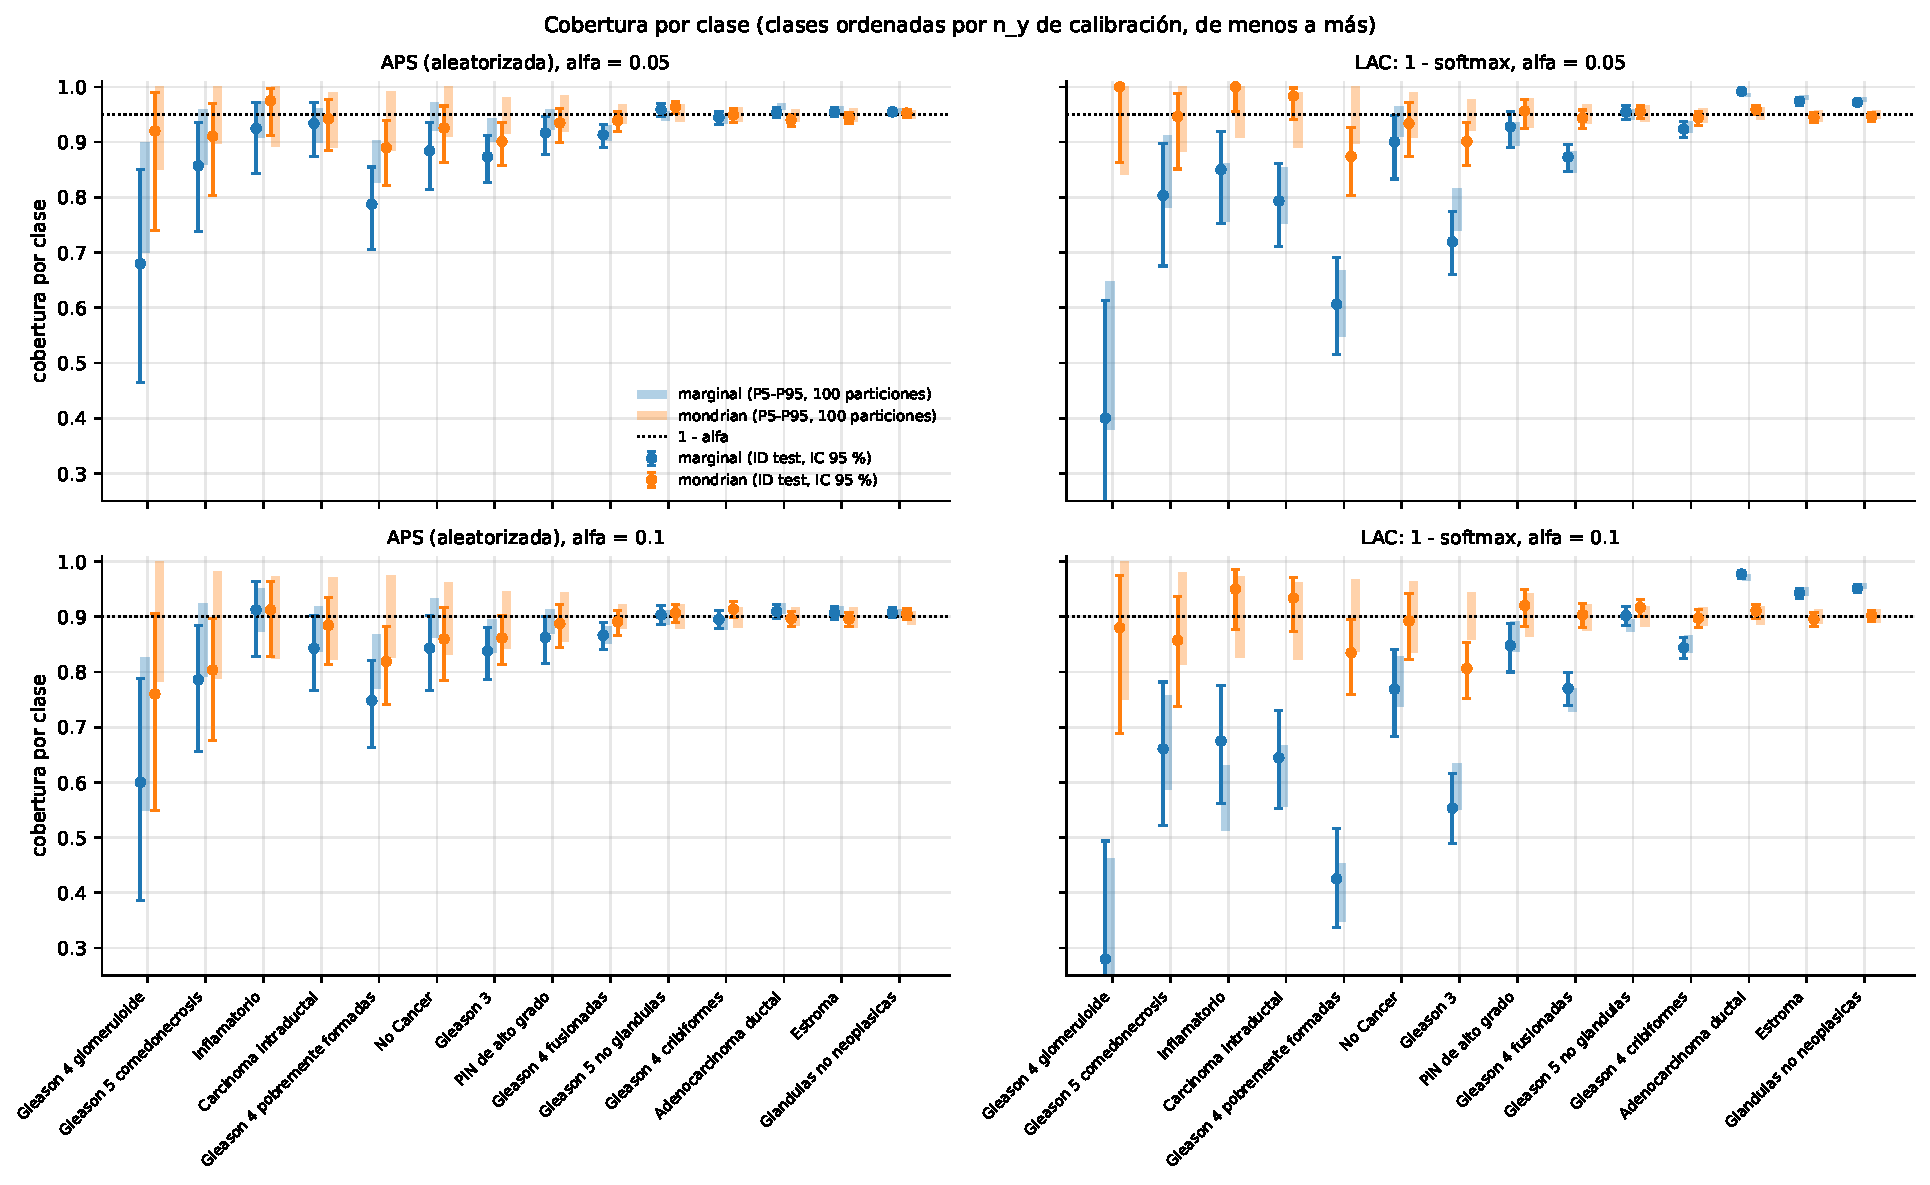
\includegraphics[width=0.85\textwidth]{img/cap12/mondrian_fig_cobertura_por_clase.pdf}
  \caption{Cobertura por clase en el test ID de la predicción conforme marginal y Mondrian.}
  \label{fig:mondrian-cobertura-clase}
\end{figure}

% Puntos que debería cubrir:
% - Mondrian coincide con la teoría en todas las clases (LAC, \alpha = 0,05): medias 0,949-0,965
%   frente a 0,950-0,966 teóricas.
% - La versión marginal infracubre sistemáticamente las clases pequeñas (glomeruloide 0,51 [0,38;
%   0,65]).
% - En el test, la cobertura Mondrian de pobremente formadas (0,874) y Gleason_3 (0,901) queda por
%   debajo del P5 de las particiones (0,897 y 0,921): evidencia de que validación y test no son
%   intercambiables en esas clases.
\pendiente{análisis de la \cref{fig:mondrian-beta}}

\begin{figure}[tbp]
  \centering
  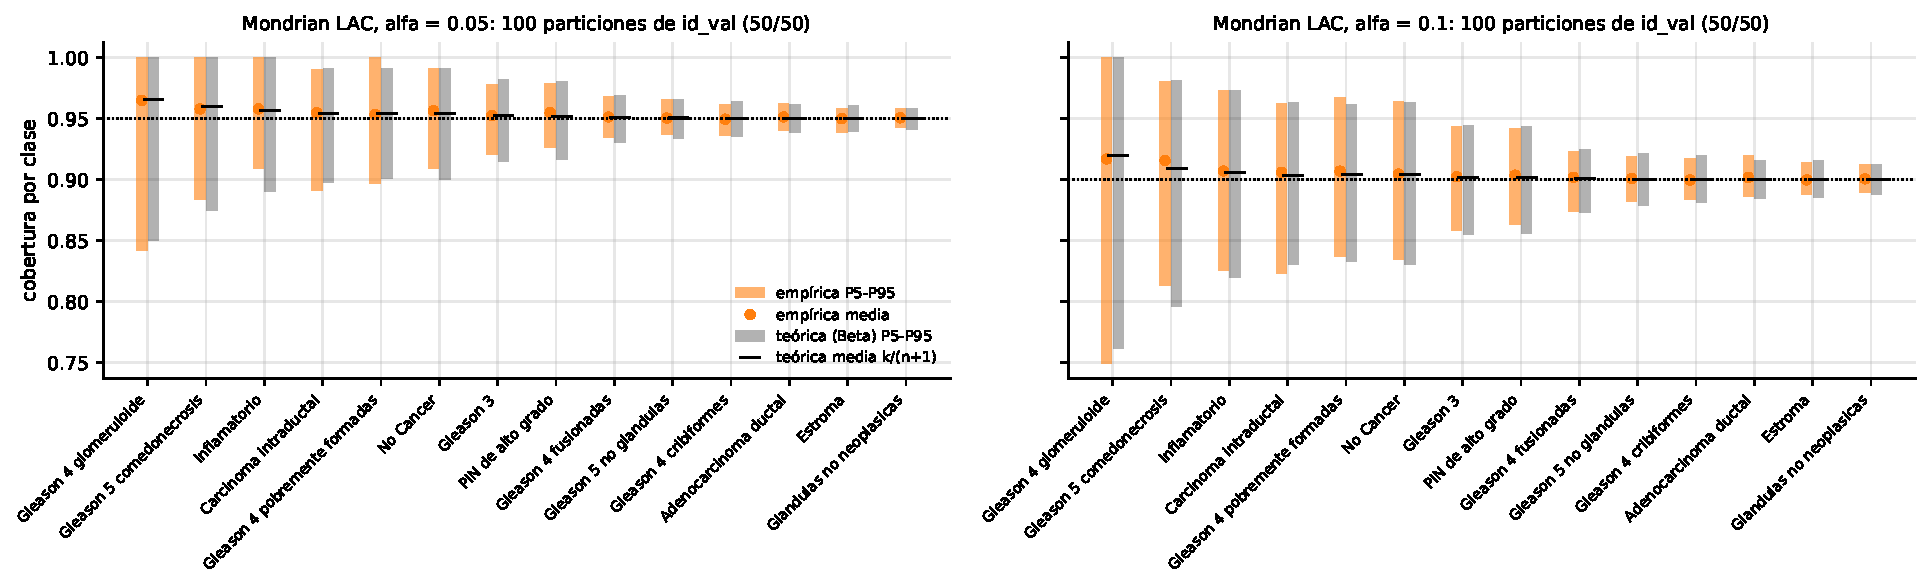
\includegraphics[width=0.85\textwidth]{img/cap12/mondrian_fig_variabilidad_vs_beta.pdf}
  \caption{Cobertura por clase en 100 particiones aleatorias de la validación ID (50\,\% calibración, 50\,\% evaluación) frente a la distribución teórica $\mathrm{Beta}(k_y, n_y + 1 - k_y)$.}
  \label{fig:mondrian-beta}
\end{figure}

% Puntos que debería cubrir:
% - Con 33 imágenes de calibración, el umbral de glomeruloide es el máximo (\cref{prop:mondrian-ny}):
%   \hat q_y = 0,995 (LAC), es decir, la clase entra si su softmax es \ge 0,005, lo que ocurre en el
%   99,2 % del test ID. Sin esa clase, el tamaño medio sería 0,99. Lo fija una sola imagen
%   (1449718_015457_039873_000224.png, predicha como cribiforme con 0,921).
% - Label smoothing (\varepsilon = 0,1, \cref{prop:ls-optimo}): el óptimo da \varepsilon/K = 0,00714 a las
%   clases no verdaderas; en el test, mediana 0,00682 y el 98,1 % entre \varepsilon/(2K) y 2\varepsilon/K.
% - Con \alpha = 0,10 el efecto desaparece (glomeruloide en el 2,3 % de los conjuntos).
\pendiente{análisis de la \cref{fig:mondrian-glomeruloide}}

\begin{figure}[tbp]
  \centering
  \begin{subfigure}[b]{0.48\textwidth}
    \centering
    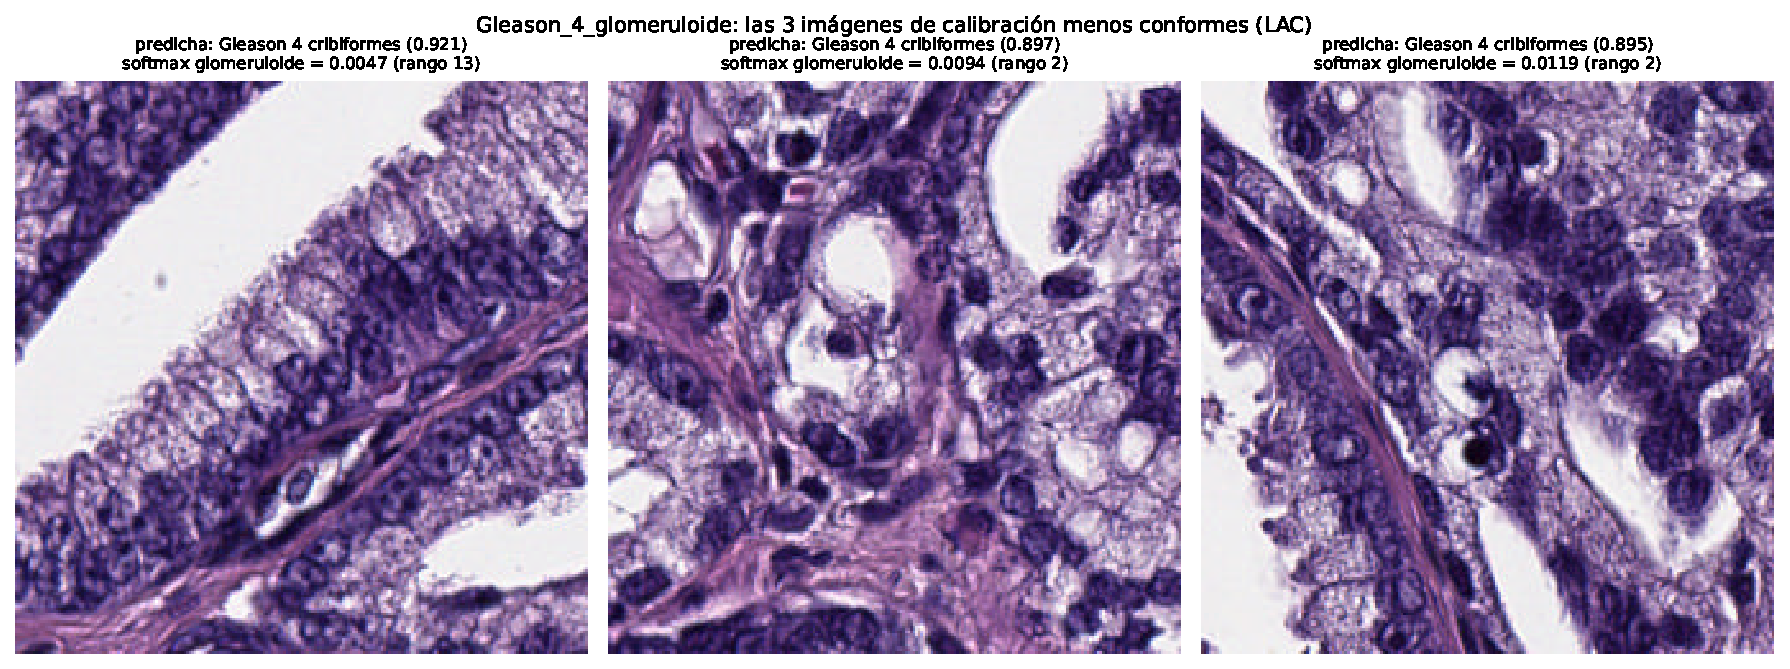
\includegraphics[width=\textwidth]{img/cap12/mondrian_fig_glomeruloide_calibracion.pdf}
    \caption{Imágenes de calibración que fijan el umbral de \clase{Gleason\_4\_glomeruloide}.}
  \end{subfigure}
  \hfill
  \begin{subfigure}[b]{0.48\textwidth}
    \centering
    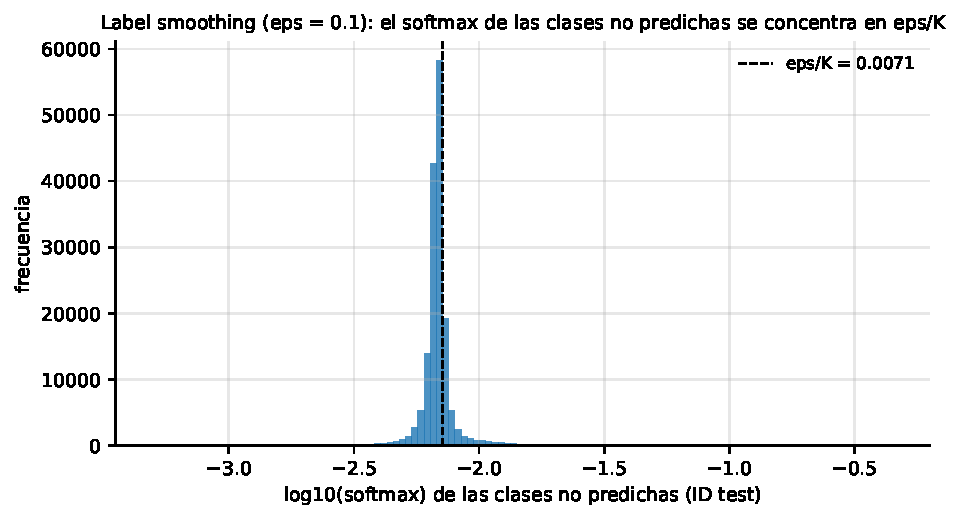
\includegraphics[width=\textwidth]{img/cap12/mondrian_fig_label_smoothing.pdf}
    \caption{Distribución del softmax de las clases no predichas y «suelo» $\varepsilon/K$.}
  \end{subfigure}
  \caption{Causa del aumento del tamaño de los conjuntos con Mondrian y $\alpha = 0{,}05$.}
  \label{fig:mondrian-glomeruloide}
\end{figure}

\pendiente{conclusión parcial}

\section{Discusión}\label{sec:conforme-discusion}

% Integrar: la detección OOD conforme controla las falsas alarmas; los conjuntos APS ofrecen
% cobertura marginal y su tamaño señala OOD; Mondrian corrige la infracobertura de las clases
% minoritarias con dos costes (conjuntos mayores con clases muy pequeñas y fragilidad ante
% covariate shift con LAC); la no intercambiabilidad entre validación y test limita las garantías.
\pendiente{discusión global}

\endinput
